\documentclass{standalone}
\usepackage{tkz-fct}
\usepackage{tkz-euclide}
\usepackage{amsmath}
\usepackage{color}
\renewcommand*\familydefault{\sfdefault}
\usepackage{sansmath}
\sansmath
\renewcommand{\arraystretch}{1.6}
\definecolor{gray75}{gray}{0.75}
\begin{document}
 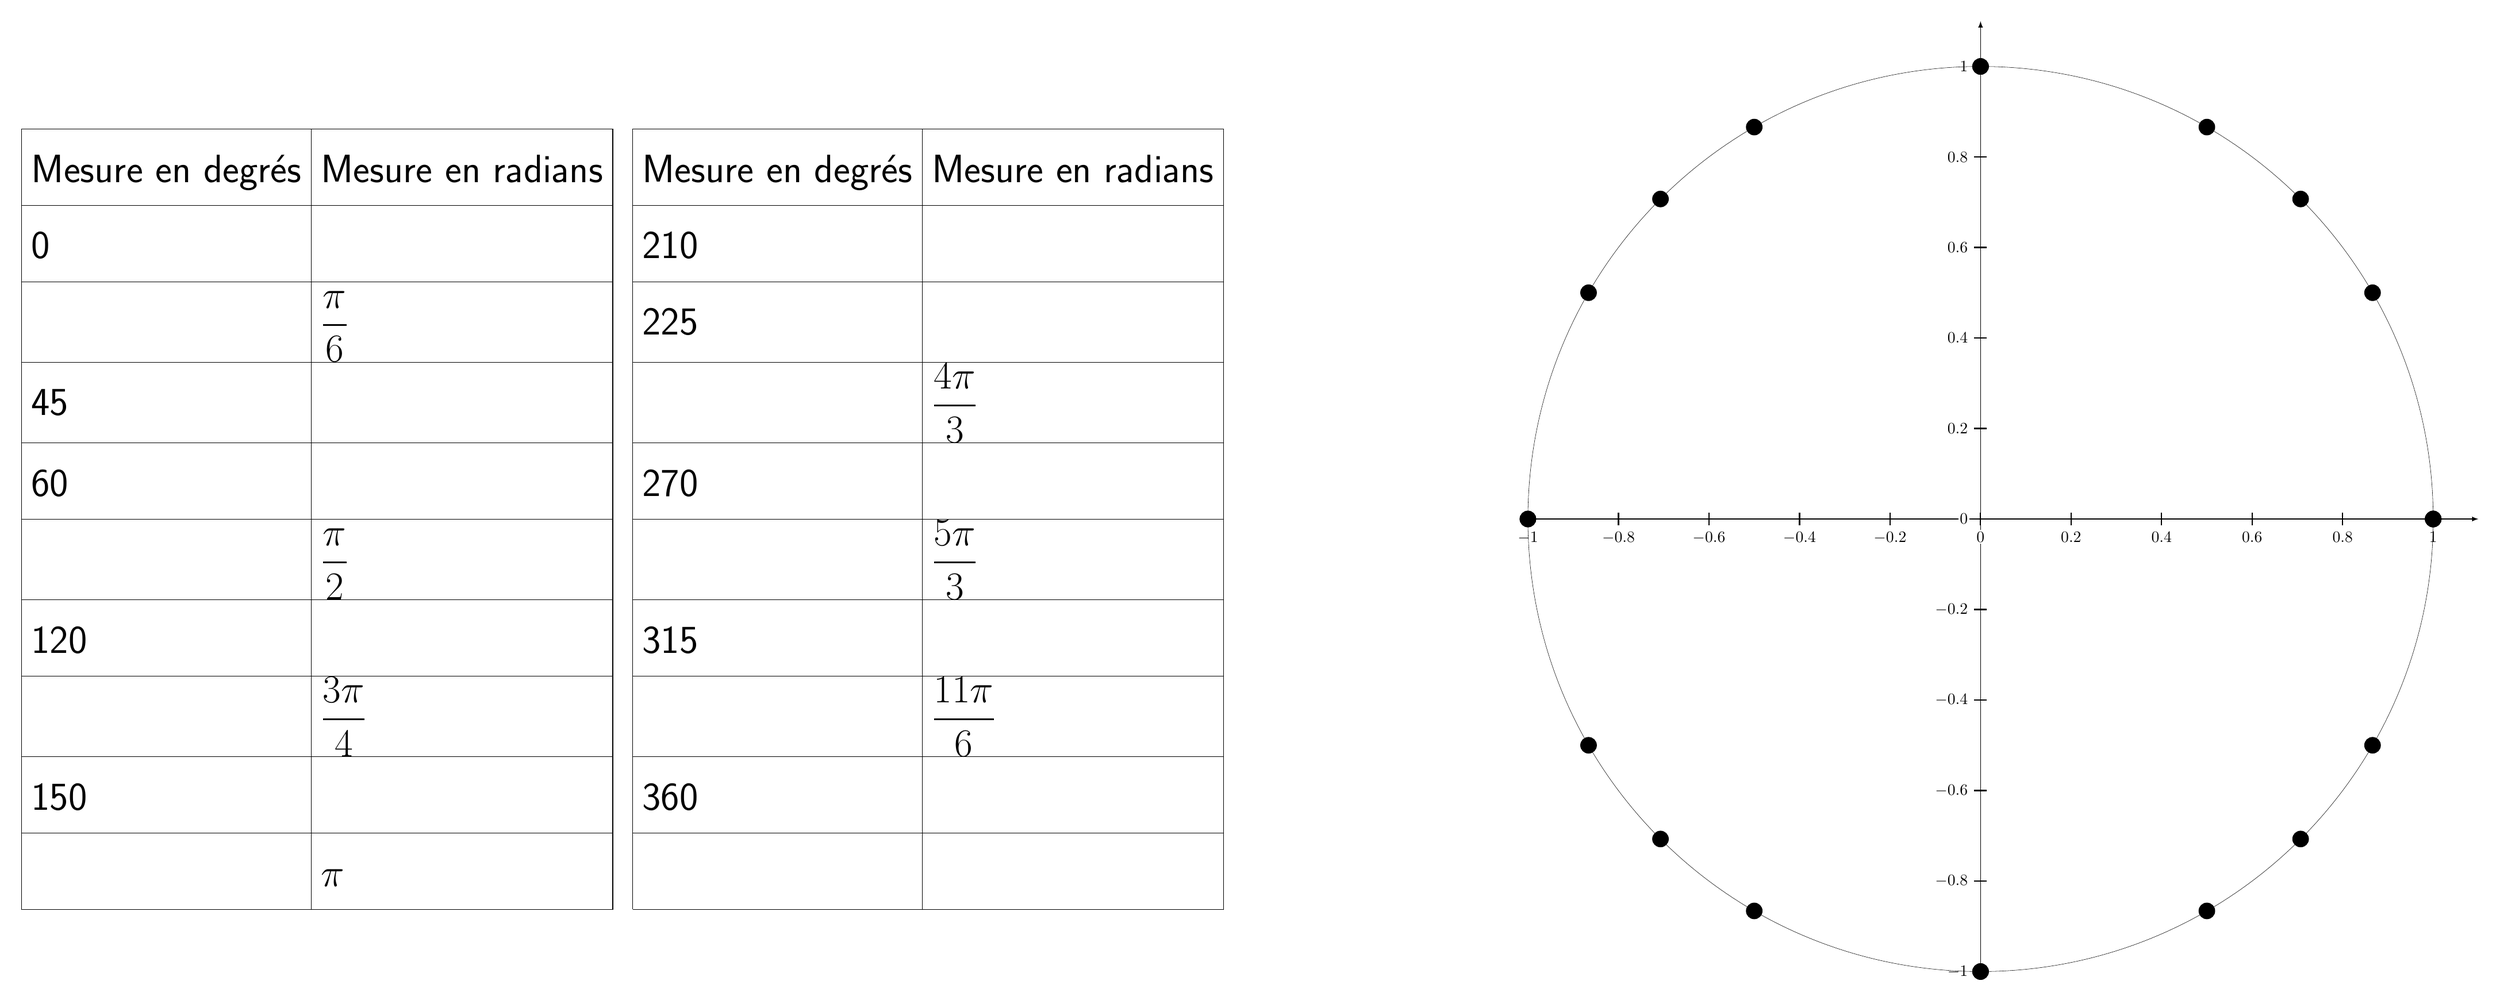
\begin{tikzpicture}[scale=2]
   \tkzInit[xmax=1.,ymax=1.,xmin=-1. ,ymin=-1,xstep=0.2,ystep=0.2]
   \tkzAxeXY[label={}]
   % \begin{scope}[dashed]
   %   \tkzGrid
   % \end{scope}

   \tkzDefPoints{0/0/O,1/0/A}
   \tkzDrawCircle[color=black](O,A)
   \foreach \a in {0,30,60,...,360}{%
     \tkzDefPointBy[rotation= center O angle \a](A)
     \tkzGetPoint{a}
     \tkzDrawPoint[size=10](a)
   }
   \foreach \a in {0,45,...,360}{%
     \tkzDefPointBy[rotation= center O angle \a](A)
     \tkzGetPoint{a}
     \tkzDrawPoint[size=10](a)
   }
\tkzText(-3,0){\Huge
\begin{tabular}{|l|l|l|l|l|}
\cline{1-2} \cline{4-5}
Mesure en degrés & Mesure en radians &  & Mesure en degrés & Mesure en radians  \\ \cline{1-2} \cline{4-5}
0                &                   &  & 210              &                    \\ \cline{1-2} \cline{4-5}
                 & $\dfrac{\pi}{6}$  &  & 225              &                    \\ \cline{1-2} \cline{4-5}
45               &                   &  &                  & $\dfrac{4\pi}{3}$  \\ \cline{1-2} \cline{4-5}
60               &                   &  & 270              &                    \\ \cline{1-2} \cline{4-5}
                 & $\dfrac{\pi}{2}$  &  &                  & $\dfrac{5\pi}{3}$  \\ \cline{1-2} \cline{4-5}
120              &                   &  & 315              &                    \\ \cline{1-2} \cline{4-5}
                 & $\dfrac{3\pi}{4}$ &  &                  & $\dfrac{11\pi}{6}$ \\ \cline{1-2} \cline{4-5}
150              &                   &  & 360              &                    \\ \cline{1-2} \cline{4-5}
                 & $\pi$             &  &                  &                    \\ \cline{1-2} \cline{4-5}
\end{tabular}
}
\end{tikzpicture}
\end{document}
